All results presented below can be reproduced by following the lab on
the following publicly available repository:
\footnote{\url{https://gitlab.inria.fr/VeRDi-project/madeus-journal}}

%--------------------------------------
\subsection{Prototype implementation details}
The prototype implementation was made in \python. As already
illustrated in Listings~\ref{codemdb}, \ref{codeapache}
and~\ref{codeass}, \mad' users declare components by creating a class,
inheriting from the internal \emph{Component} class, containing the
description of the \net as well as the actions associated to the
transitions. These actions are \python functions which usually perform
remote actions using SSH, Ansible or other tools. Users can then
create an assembly by extending the appropriate class and listing the
components and how their ports are connected. This assembly can then
be run, which means that the semantics of Madeus is executed in this
assembly. The commissioning is over if the only elements holding a
token are places without outgoing transitions. While this is not the
case, the semantics is executed by attempting to apply each rule from
the semantics on each component. When a transition is fired, the
corresponding \python function is executed in a Python thread, which
does not block the execution of the semantics. Note that \python
threads do not take advantage of hardware parallelism capabilities,
but because the functions usually run other (possibly remote)
processes to do the heavy work, this is not an issue. The
$\terminaction$ rule can be executed for the corresponding function
when it has finished its execution.

% --------------------------------------
\subsection{Results}

Madeus is a model that relies on the description of a control
component for each software module of that will be deployed. It is a
low-level model, therefore the developer is responsible for the
choices of actions performed in the transitions.  This section
evaluates the performance of Madeus' prototype with empty transitions
in order to evaluate the \mad prototype independently of any specific
transitions. This is why these experiments are called
\emph{dry-runs}. It means the transitions do not contain any code or
command for which the execution time is unknown or imprecise, thus
allowing to measure the overhead caused by the prototype only. In
addition to this, the experiments presented in this section are
compared to the theoretical performance computed by the prediction
model detailed in Section~\ref{sec:perf_model}. By doing so we both
validate the theoretical performance model compared to the reality,
and the expected performance of the prototype on the set of use-cases.

% figures to add for assemblies
%Sequential

\begin{figure}[h]
  \begin{center}
    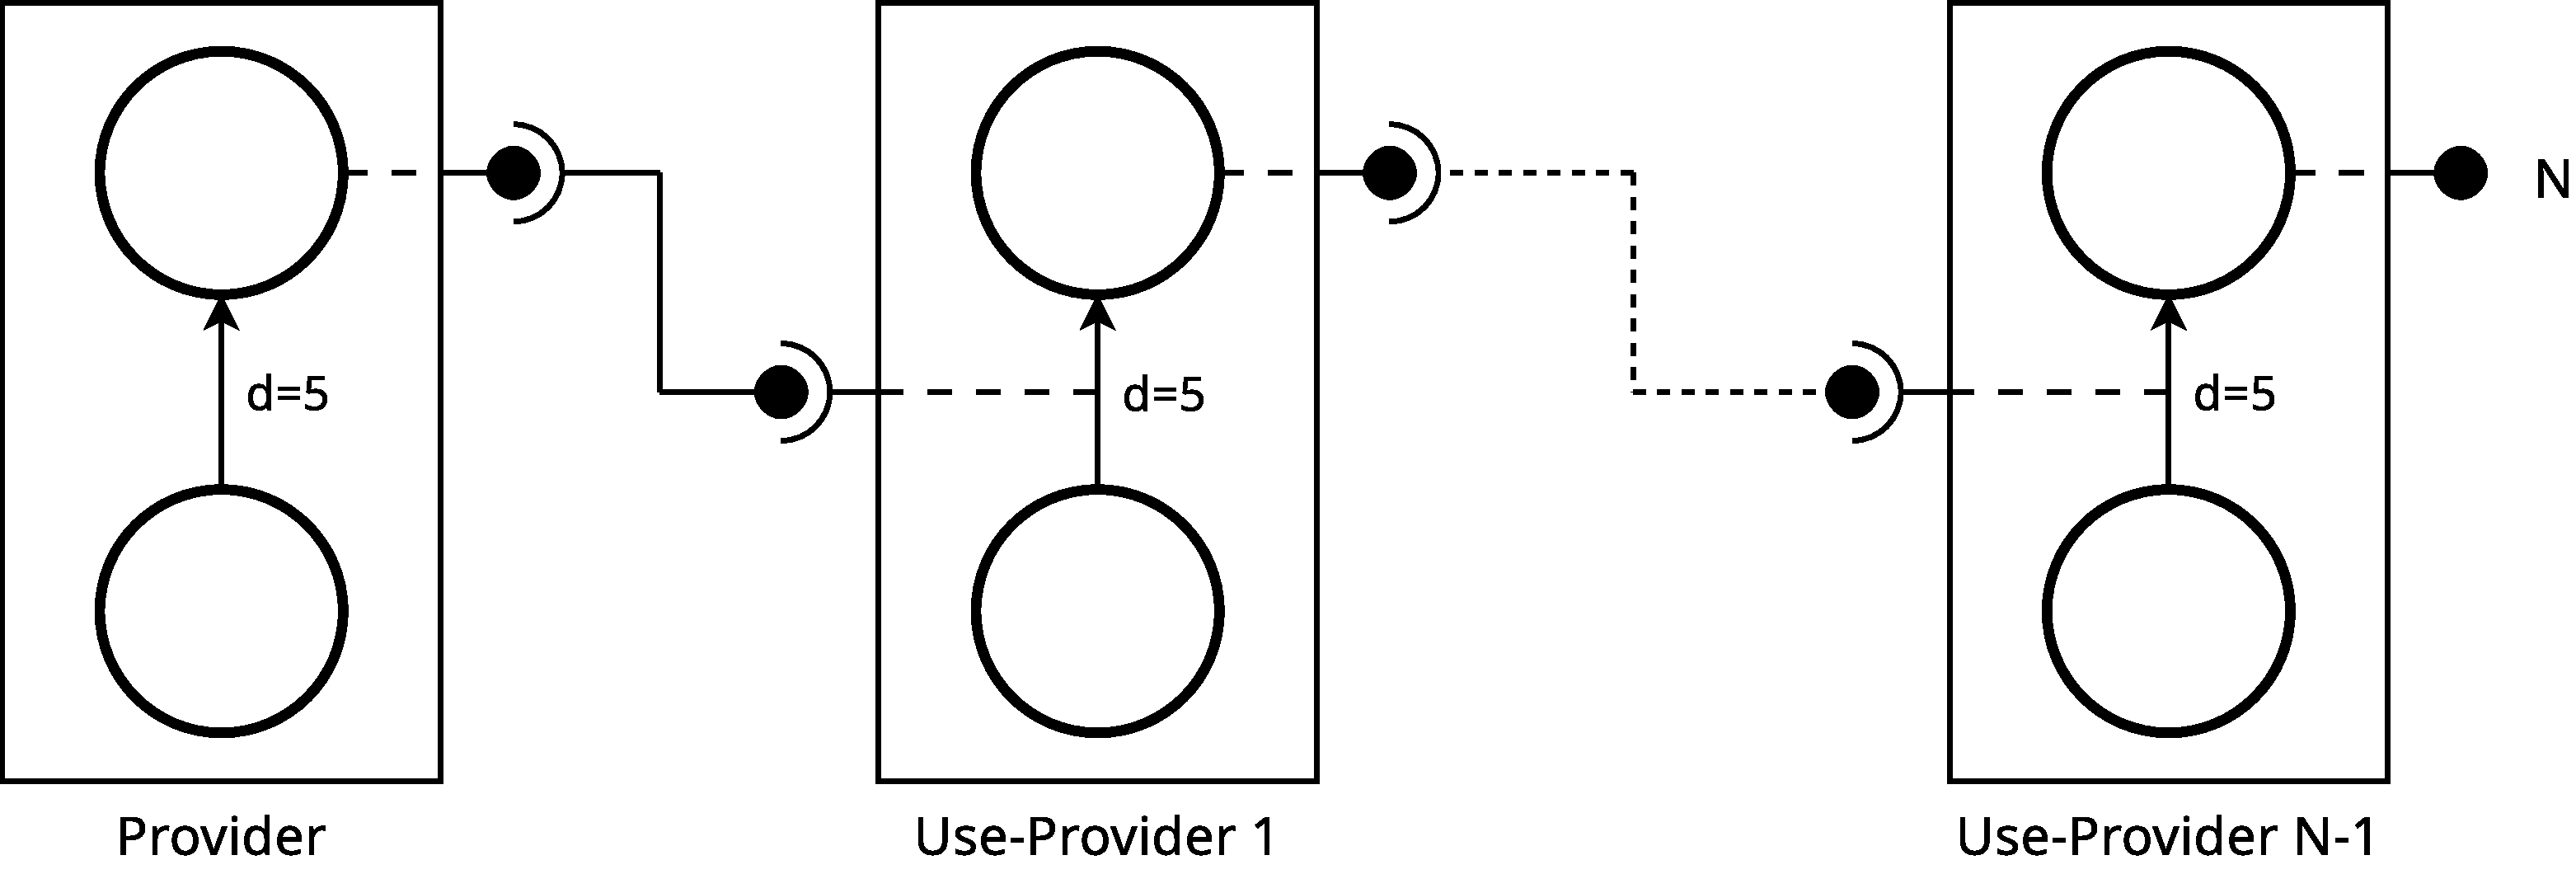
\includegraphics[width=0.4\textwidth]{./images/seq.pdf}
    \caption{The \mad sequential assembly of Benchmark (A), with N components.}
    \label{fig:seq}
  \end{center}
\end{figure}

Three benchmarks compose this evaluation and are illustrated in
Figures~\ref{fig:seq} and~\ref{fig:par}.
% first
The first benchmark, denoted (A), models a sequential \mad assembly,
depicted in Figure~\ref{fig:seq}. It is composed of one
\emph{provider} component made of a transition and two places, and
$N-1$ \emph{user-provider} components that are also composed of a
transition and two places, but where the transition uses the provide
port of the preceeding component. The components are connected in
chain thus resulting in a sequential execution.
%The dry-run version of
%this assembly consists in transitions that do nothing besides wait for
%a fixed amount of time.
%The second version of this assembly features a transition that calls
%an ssh connection and waits for a fixed amount of time, similar as for
%the dry-run version, before finishing.

\begin{figure}[h]
  \begin{center}
    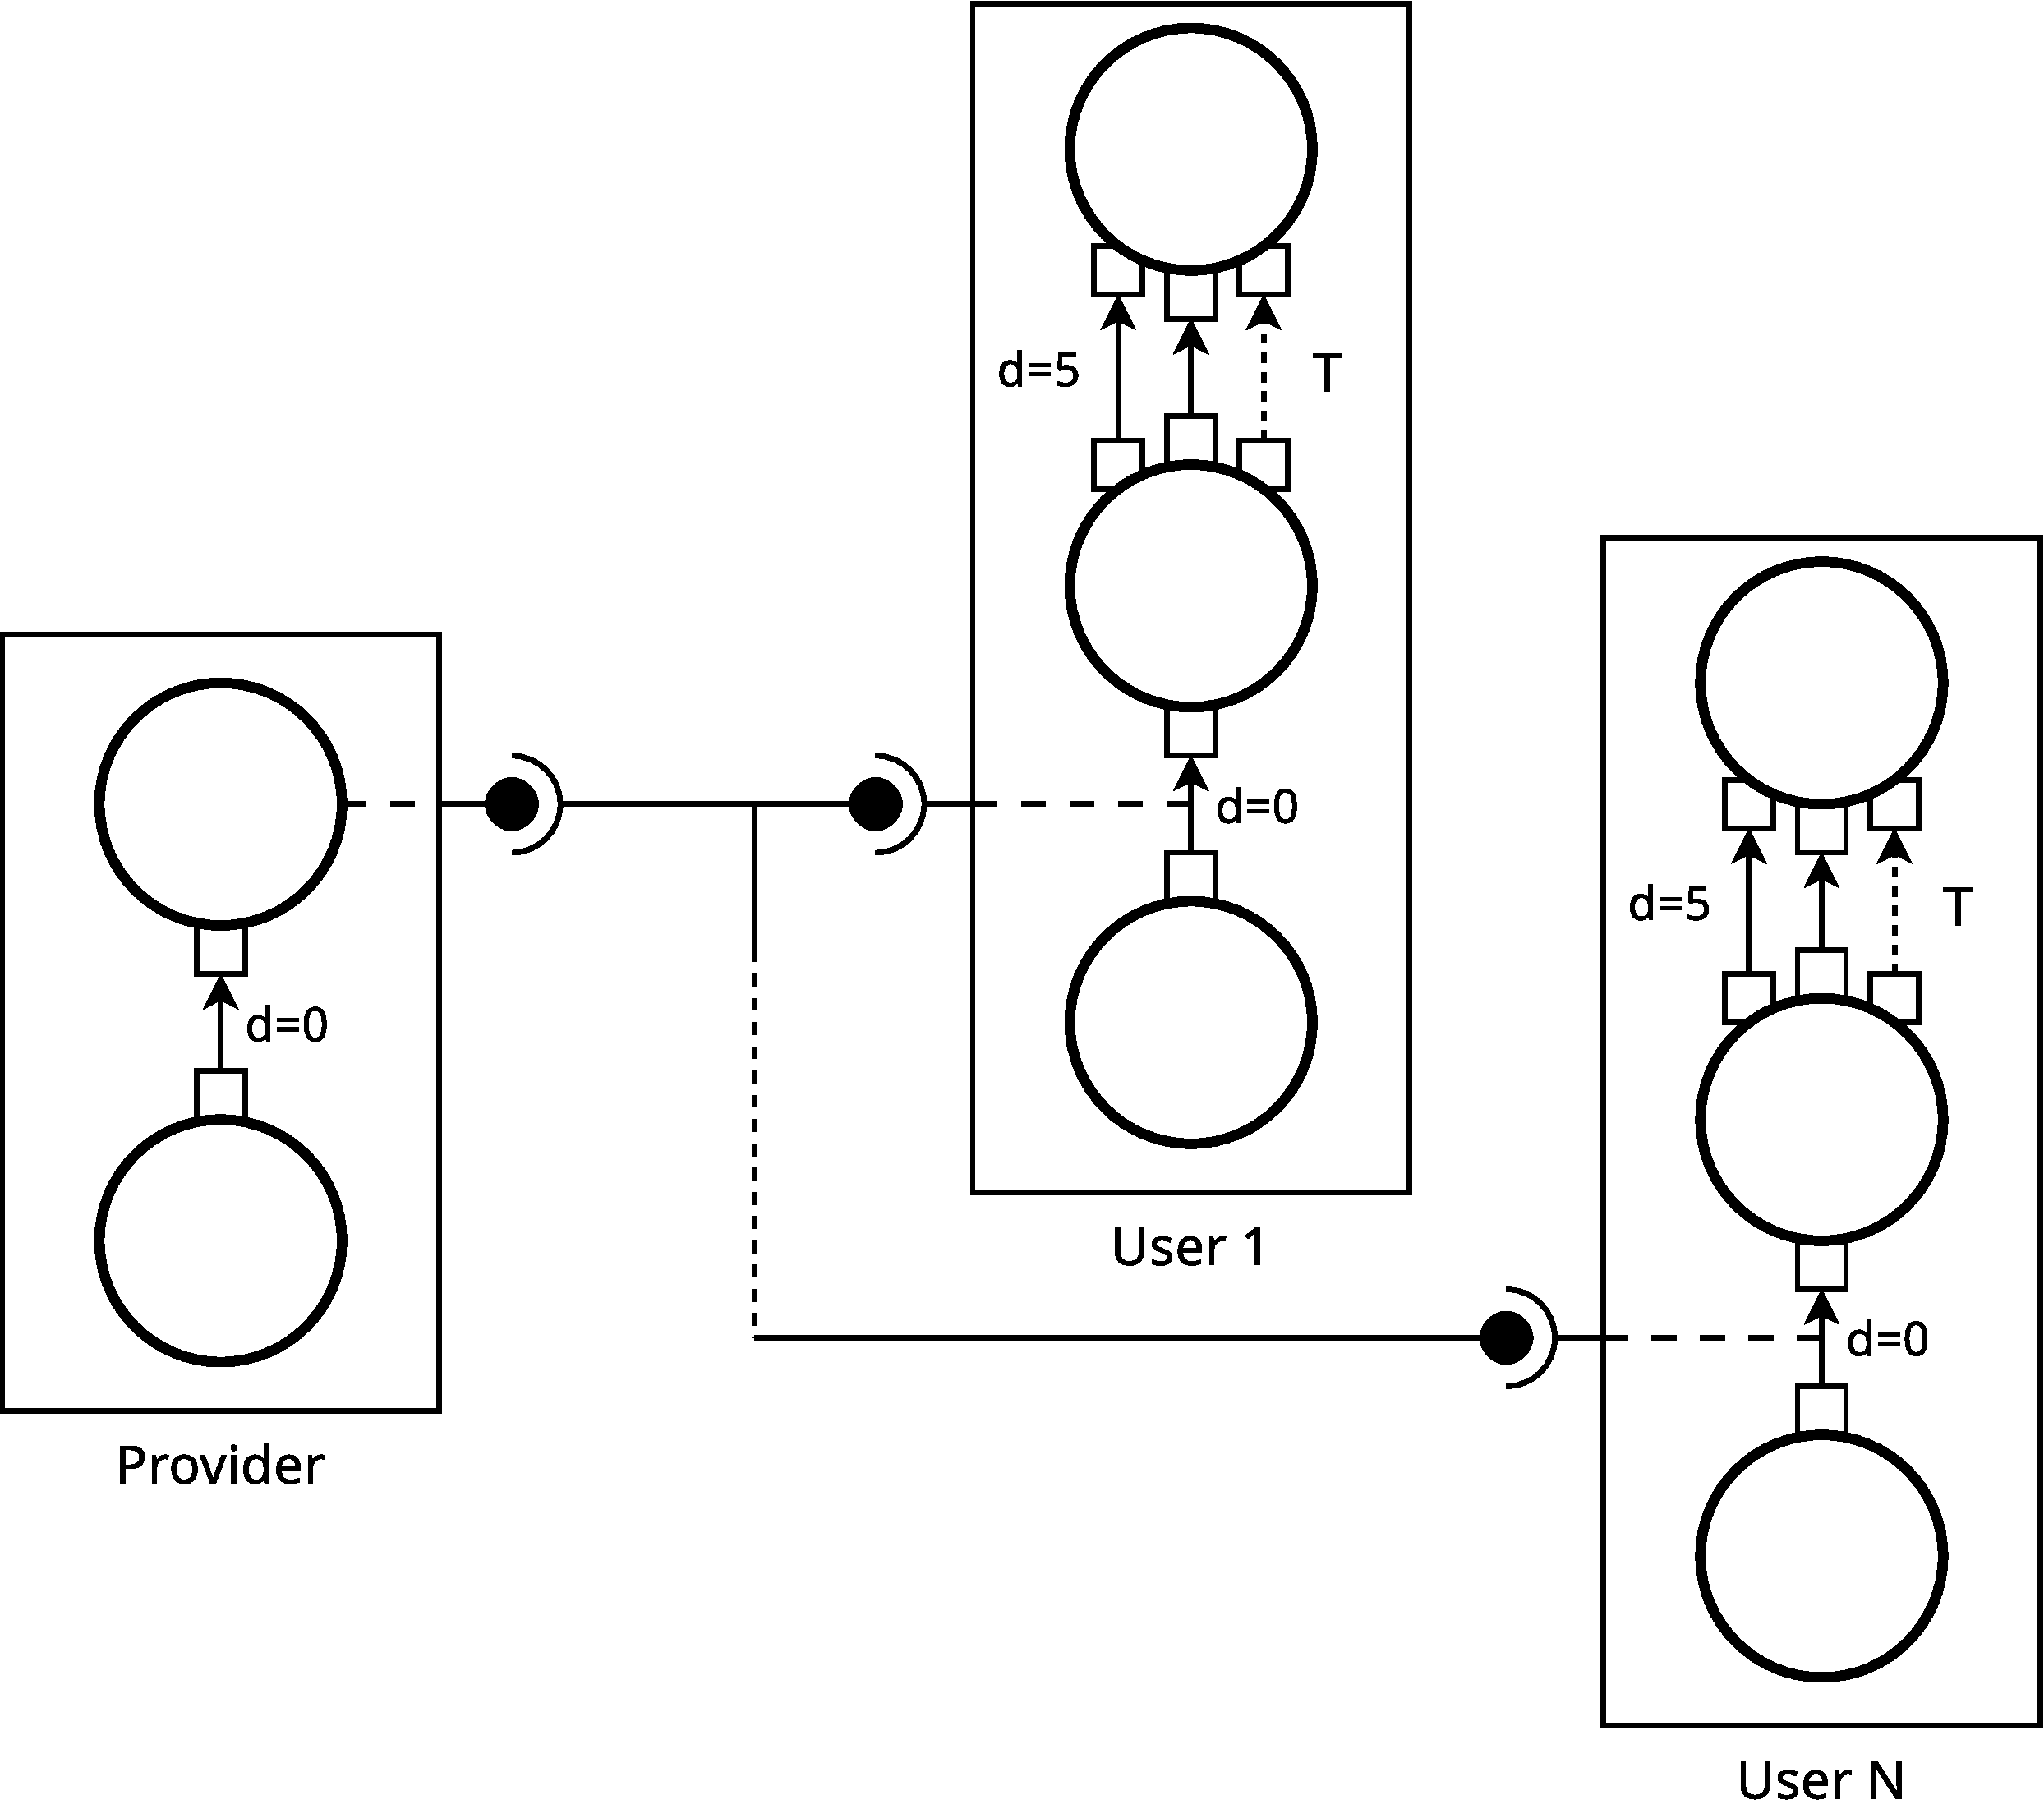
\includegraphics[width=0.4\textwidth]{./images/par.pdf}
    \caption{The \mad parallel assembly of Benchmark (B) and (C), with N parallel components, and T parallel transitions.}
    \label{fig:par}
  \end{center}
\end{figure}

%second
The two other benchmarks model \mad parallel assemblies and are
depicted in Figure~\ref{fig:par}. The first assembly, denoted (B)
evaluates the parallelism at the component level, called
\emph{inter-comp} and \emph{inter-comp-tasks}. The second one, denoted
(C), models the parallelism at the transition level, \ie
\emph{intra-comp-tasks}, when transitions are performed
simultaneously.
%
Both benchmarks use the same assembly that is composed of an initial
\emph{provider} component and $N$ parallel \emph{user} components
connected to the provider. Each \emph{user} component contains a first
transition that uses the service provided by the provider component
and $T$ parallel transitions. For Benchmark (B), the number of
components varies from 1 to 40 components with a single transition per
component $T=1$. For Benchmark (C), the number of component is fixed
to $N-1=1$ and the number of transitions varies from 1 to 20.

Experiments have been performed on a single node of the \ecotype
cluster of the experimental platform
Grid'5000\footnote{\url{www.grid5000.fr}}. The detailed configuration
of the node is given in Table~\ref{tab:g5k}. Each experiment presented
in the results is an average of ten executions. The duration of some
transitions of the benchmarks are set to $d=0$ and the transitions
that are interesting for the results are set to $d=5$ (seconds). This
execution time is guaranteed by the call to the sleep function of
\python. This execution time has been chosen to get a coherent and
readable scale of results.
%They are both evaluated in \emph{dryrun} mode without any
%ssh connections and with \emph{ssh connections} active in the assembly
%between components, so as to allow visualisation of the eventual
%overhead of having these ssh connections.

\begin{figure}[h]
  \begin{center} 
    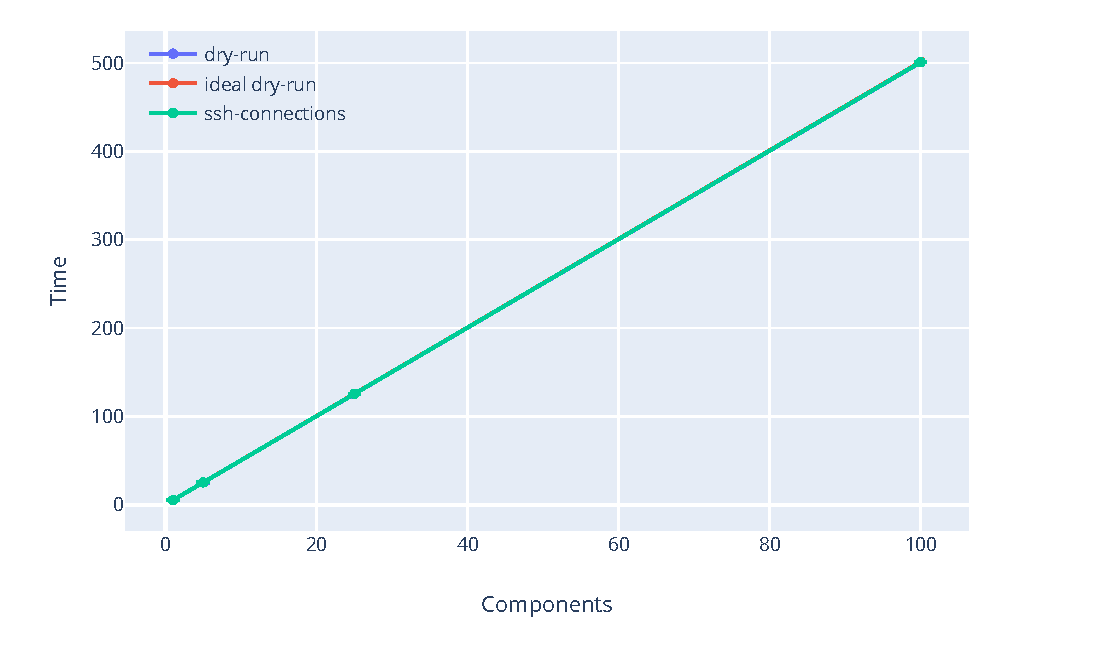
\includegraphics[width=0.5\textwidth]{./images/evaluations_sequential.pdf}
    \caption{Results of the sequential benchmark.}
    \label{fig:seqres}
  \end{center}
\end{figure}

Figure~\ref{fig:seqres} presents the results of Benchmark (A). As (A)
models a sequential assembly, the theoretical execution time is simply
the sum of the execution time of each transition of each component
($N$ components). The results show a linear increase in time and the
\emph{dryrun} curve follows the \emph{ideal} curve closely.
%The difference between the
%\emph{ssh-connections} curve is hard to visualise but is slightly
%higher than the \emph{ideal} and \emph{dryrun} curves, a logical
%result as the number of ssh connections grows with each component
%added, but there is always only one ssh connection at the same time.

\begin{figure}[h]
  \begin{center} 
    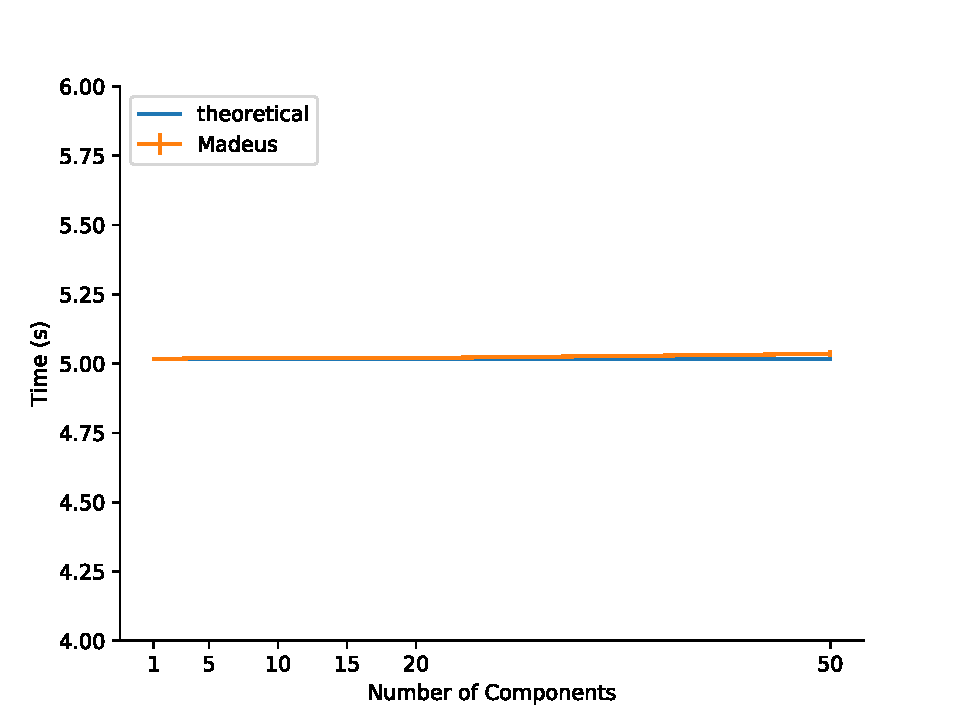
\includegraphics[width=0.5\textwidth]{./images/evaluations_par_component.pdf}
    \caption{Results of the parallel assembly benchmark with varying component number}
    \label{fig:parcompres}
  \end{center}
\end{figure}

% attention à comprendre si c'est systématique !
%For the results on the parallel assembly benchmark, we had to remove
%one outlier data point on the parallel assembly benchmark for
%component parallelism, as the first iteration of the assembly with
%just one component always had 4 seconds added to the time and we could
%not pinpoint the exact reason for that. As it did not occur for any of
%the other iterations, we did not take it into account on the curve
%drawing for our Figure~\ref{fig:parcompres}. In the results directory
%that can be found on our repository we have included the original
%times.json and the modified times.json files to keep the original
%results intact.

Figure~\ref{fig:parcompres} depicts the results of Benchmark (B). The
ideal theoretical performance for this benchmark is a constant equal
to the duration time of the main transition of \emph{user} components,
\ie $5$ seconds. Indeed as components are independent from each other
(no ports) they are deployed simultaneously.
%value as components are commissioned in parallel. In \emph{dryrun}
%our experimental benchmark
One can note that the results observed with the \mad prototype is only
very slightly above the ideal constant result, which shows that the
prototype does not add significant overhead to the process even for a
large number of parallel components on the same node. Indeed,
deploying 40 components or services on a single node is unusual.
%The \emph{ssh connection} curve allows us to see
%that there is steady increase of time, adding almost 3 seconds to the
%assembly deployment when reaching 40 parallel components. This show
%that the overhead added by the SSH connections is not null.

\begin{figure}[h]
  \begin{center} 
    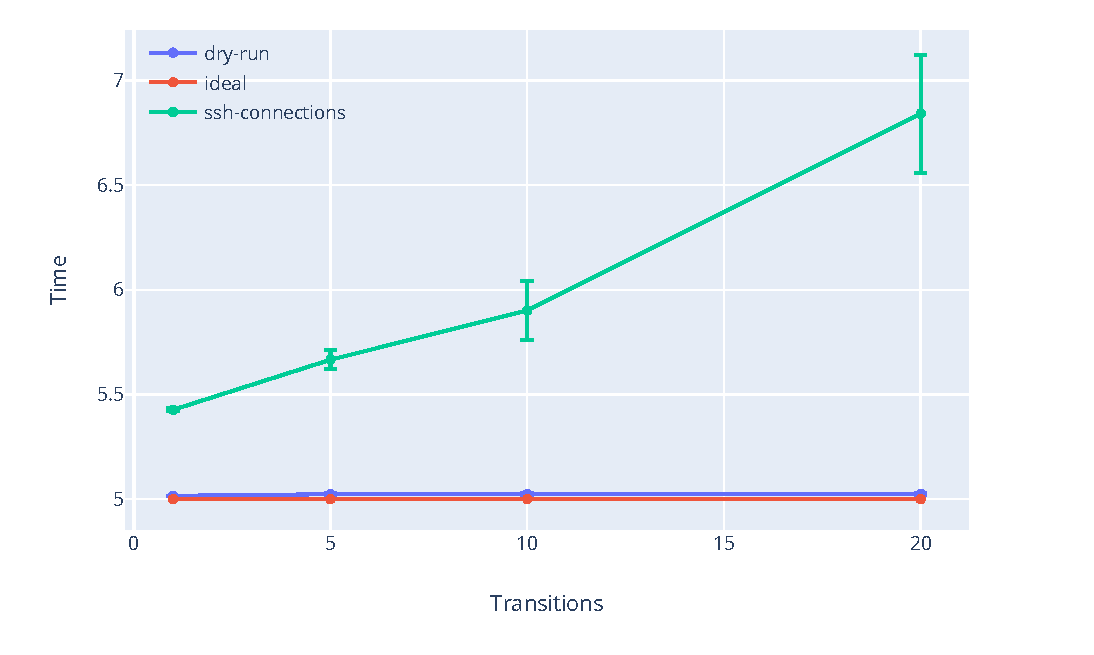
\includegraphics[width=0.5\textwidth]{./images/evaluations_par_transitions.pdf}
    \caption{Results of the parallel assembly benchmark with varying parallel transition number}
    \label{fig:partrans}
  \end{center}
\end{figure}

Figure~\ref{fig:partrans} shows the results for Benchmark (C). As for
the previous benchmark, and because transitions are executed
simultaneously in this benchmark, the theoretical expected curve is a
constant equal to the duration time of one of the $T$ transitions, \ie
$5$ seconds. The results follow the ideal curve closely as well for a
large number of transitions.

%calculation for the ideal curve on the parallel assembly benchmark
%when varying the number of parallel transitions has been done in the
%same manner as for the parallel component variation. In \emph{dryrun}
%the benchmark results follow the ideal curve closely as well, whereas
%the \emph{ssh connections} curve has an overhead that grows as the
%number of transitions increases.

These results allow us to point out that \mad does not by itself add a
big overhead on the deployment. One can note though that according to
the type of commands performed in the transitions  an additional
overhead could be observed. For instance, .
\HC[Helene]{est-ce que c'est utile de donner l'exemple du surcoût SSH ?}
%They also show the
%importance of ssh connection and their impact on the deployment time.


